\documentclass[12 pt, a4paper]{report}
%\documentclass[runningheads]{llncs}
\usepackage[T1]{fontenc}
\usepackage{mathptmx}
\usepackage{amsmath,amssymb,amsfonts, amsthm}

\theoremstyle{definition}
\newtheorem{definition}{Definition}[section]

\usepackage{setspace}
%\usepackage[top=1 in,bottom=1 in,left=3.2 cm,right=2.6 cm]{geometry}
\usepackage[utf8]{inputenc}
\usepackage{fullpage}
\usepackage{graphicx}
%\renewcommand{\baselinestretch}{2}
%\renewcommand{\thesection}{\arabic{section}}
%\raggedbottom
\usepackage[sort&compress,numbers]{natbib}
\usepackage[hidelinks]{hyperref}
\usepackage[nottoc]{tocbibind}
\usepackage{rotating}
\usepackage{hyperref}
\usepackage{lipsum}
\usepackage{xcolor}
%\usepackage{afterpage}
\usepackage{parskip} 
%removes indentation but gives some spacing ebtween para
\usepackage{todonotes}
\usepackage[toc,acronym]{glossaries}

\usepackage{booktabs}
%\usepackage{minted}
\usepackage{listings}

\definecolor{codegreen}{rgb}{0,0.6,0}
\definecolor{codegray}{rgb}{0.5,0.5,0.5}
\definecolor{codepurple}{rgb}{0.58,0,0.82}
\definecolor{backcolour}{rgb}{0.90,0.90,0.90}

\lstdefinestyle{mystyle}{
    backgroundcolor=\color{backcolour},   
%    commentstyle=\color{codegreen},
    keywordstyle=\color{magenta},
    numberstyle=\tiny\color{codegray},
%    stringstyle=\color{codepurple},
    basicstyle=\ttfamily\scriptsize,
    breakatwhitespace=false,         
    breaklines=true,                 
    captionpos=b,                    
    keepspaces=true,                 
    numbers=none,                    
    numbersep=5pt,                  
    showspaces=false,                
    showstringspaces=false,
    showtabs=false,                  
    tabsize=2,
    escapechar=\%,
    framexleftmargin=5mm,
    frame=single,
    rulecolor=\color{black}
%    flexiblecolumns=true	
}

\lstset{style=mystyle}



\newcommand{\blankpage}{
\newpage
\thispagestyle{empty}
\addtocounter{page}{-1}
\mbox{}
\newpage
}

%\newcommand\blankpage{%
%    \null
%    \thispagestyle{empty}%
%    \addtocounter{page}{-1}%
%    \newpage}

%\def\keywords{\vspace{.5em}
%{\textit{Keywords}:\,\relax%
%}}
%\def\endkeywords{\par}

%\providecommand{\keywords}[1]
%{
%  \small	
%  \textbf{\textit{Keywords---}} #1
%}

\counterwithout{footnote}{chapter}

\makeglossaries

\makeglossaries
\newglossaryentry{wd}
{
    name=wd,
    description={Is the prefix for the namespace - http://www.wikidata.org/entity used for items in Wikidata}
}

\newglossaryentry{wdt}
{
    name=wdt,
    description={Is the prefix for the namespace - http://www.wikidata.org/prop/direct/ used for properties in Wikidata}
}

\newglossaryentry{rdf}
{
    name=rdf,
    description={Is the prefix for the namespace - http://www.w3.org/1999/02/22-rdf-syntax-ns\# used in RDF}
}

\newglossaryentry{rdfs}
{
    name=rdfs,
    description={Is the for the namespace - http://www.w3.org/2000/01/rdf-schema\# where the core vocabulary of RDF is defined}
}

\newglossaryentry{xsd}
{
    name=xsd,
    description={Is the prefix for the namespace - http://www.w3.org/2001/XMLSchema\# which is the XML Schema that defines the datatypes}
}

\newglossaryentry{Q560}
{
    name=Q560,
    description={Is the ID for the item "Helium" in Wikidata}
}

\newglossaryentry{Q11344}
{
    name=Q11344,
    description={Is the ID for the item "chemical element" in Wikidata}
}

\newglossaryentry{Q298581}
{
    name=Q298581,
    description={Is the ID for the item "Pierre Janssen" in Wikidata}
}

\newglossaryentry{Q90}
{
    name=Q90,
    description={Is the ID for the item "Paris" in Wikidata}
}

\newglossaryentry{Q142}
{
    name=Q142,
    description={Is the ID for the item "France" in Wikidata}
}

\newglossaryentry{P31}
{
    name=P31,
    description={Is the ID for the property "instance of" in Wikidata}
}

\newglossaryentry{P2102}
{
    name=P2102,
    description={Is the ID for the property "boiling point" in Wikidata}
}

\newglossaryentry{P274}
{
    name=P274,
    description={Is the ID for the property "chemical formula" in Wikidata}
}

\newglossaryentry{P2101}
{
    name=P2101,
    description={Is the ID for the property "melting point" in Wikidata}
}

\newglossaryentry{P2054}
{
    name=P2054,
    description={Is the ID for the property "density" in Wikidata}
}

\newglossaryentry{P61}
{
    name=P61,
    description={Is the ID for the property "discoverer/inventor" in Wikidata}
}

\newglossaryentry{P625}
{
    name=P625,
    description={Is the ID for the property "place of birth" in Wikidata}
}

\newacronym{RDF}{Resource Description Framework}

\newacronym{SPARQL}{SPARQL}{SPARQL Protocol and RDF Query Language}

\newacronym{GraphQL}{GraphQL}{Graph Query Language}

\newacronym{URI}{URI}{Uniform Resource Identifier}

\newacronym{IRI}{IRI}{Internationalized Resource identifier}

\newacronym{URL}{URL}{Uniform Resource Locator}

\newacronym{BCP47}{BCP47}{Best Current Practice 47}

\newacronym{bnodes}{bnodes}{Blank node in RDF}

\newacronym{W3C}{W3C}{World Wide Web Consortium}

\onehalfspacing
\begin{document}
%\maketitle
\sloppy
\begin{titlepage}

	\begin{doublespace}

% 		\begin{flushleft} 
 
			
\includegraphics[width=0.4\textwidth]{images/logo.jpg}

			\hrule
			\vspace*{0.15cm}
			{\Large Faculty of Computer Science}
			\vspace*{0.15cm}
			\hrule

%    \begin{center}
		\begin{center}
        		\vspace{1cm}      
        
       		{\LARGE \textbf{Master Thesis} }
            
        		\vspace{0.25cm}
        
        		{\Large \textbf{Querying Wikidata with GraphQL} 
%			(Wikidata mit GraphQL Abfragen) 
			}
            
        		\vspace{1.5cm}
        \end{center}
        
        
%	 \begin{flushleft}
			Anas Shahab \\
    			Master Computational Logic \\
    			Matriculation number: 4827407
    		
    			\vspace{0.5cm}
    		
    			Supervisor: \\
	    		Prof. Dr. Markus Kr{\"otzsch}
    			
    			\vspace{0.25cm}
    		
    			Second Reviewer: \\
			Dr. Dörthe Arndt
    			
    			\vspace{0.25cm}
    		
    			
    			Tutor: \\
    			Dipl.-Inf. Lukas Gerlach
    		
    			\vspace{0.5cm}
    		
    			Faculty of Computer Science \\
    			Institute of Theoretical Computer Science \\
    			Chair of Knowledge-Based Systems
    		
    			\vspace{1cm}
    		
    			Submission Date: \textcolor{red}{XX.XX.2023}
    			
%		\end{flushleft}
                  
	\end{doublespace}
	
%	\afterpage{\blankpage}
            
%    \end{center}
\end{titlepage}
\blankpage
%\afterpage{\blankpage}

%\thispagestyle{empty}
\pagenumbering{roman}
\chapter*{Declaration of originality}
%\section*{Declaration of originality}
I hereby declare that I have written this Thesis on my own accord and any participation of others has been acknowledged. I have clearly marked all references to existing work. I have not submitted this work partly or as a whole anywhere else. \\

Dresden, XX.XX.XXXX \\
\rule{150 px}{0.5 px} \\
(signature)
\blankpage
%\afterpage{\blankpage}

%\thispagestyle{empty}
\chapter*{Acknowledgements}
%\section*{Acknowledgements}
\lipsum[1]
\blankpage

%\begin{abstract}
%\lipsum[1]
%\\[0.5 cm]
%\centerline{\keywords{x, y, z}}
%
%\end{abstract}

\chapter*{Abstract}
%\section*{Abstract}
\lipsum[1]

%\pagenumbering{roman}
\tableofcontents
%\listoffigures
%\listoftables
\pagebreak

%\doublespacing
\pagenumbering{arabic}

\chapter{Introduction}
%\section{Introduction}
\label{ch:1}
The term "knowledge graph" gained popularity in 2012 when Google launched its own "\textit{Google Knowledge Graph}". A knowledge graph is a collection of data represented as a graph. There are many ways of modelling using graphs. The most commonly used ones are directed edge-labelled graphs, heterogeneous graphs, property graphs and graph dataset \cite{Hogan2021}. In this report, we consider directed edge-labelled graphs for modelling knowledge graphs.

A directed edge-labelled graph, also known as a multi-relational graph, consists of a set of nodes and a set of directed labelled edges \cite{Hogan2021}. Information represented in knowledge graphs conveys knowledge of the real world, where the nodes represent entities of interest and the directed edges represent the many different binary relations between those entities. Entities are real world objects and abstract concepts. An object is a physical item in the real world such as a university (e.g., Technical University Dresden) or a planet (e.g., Earth). A concept on the other hand, refers to general categories of objects such as chemical element or philosopher. 

For example, the information
 \begin{verbatim}
 	\texttt{"Helium is a type of chemical element that has the chemical formula He"}
	\end{verbatim}
can be represented using a directed edge-labelled graph. The nodes of the graph would represent the entities "\texttt{Helium}", "\texttt{chemical element}" and "\texttt{He}". There would be two labelled edges, one pointing from the "\texttt{Helium}" node to the "\texttt{chemical element}" node, and the other from the "\texttt{Helium}" node to the "\texttt{He}" node. These edges would represent the relations "\texttt{instance of}" and "\texttt{chemical formula}" respectively. Figure~\ref{fig:1} shows such a directed-edge labelled graph. We provide a more complex example later in Chapter~\ref{ch:2}.

\begin{figure}[b!tp]
  \centering
  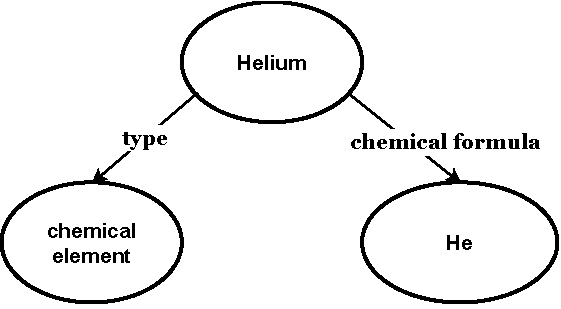
\includegraphics[width=0.75 \linewidth]{images/knowledge_graph.drawio.pdf}
  \caption{A directed-edge labelled graph}
  \label{fig:1}
\end{figure}

Resource Description Framework (RDF) \cite{R.Cyganiak2014} is a standard framework that models the Semantic Web. Its data model is based on directed edge-labelled graphs and is composed of a set of triples or statements. Each triple consist of a subject node, predicate edge and an object node. The subject and object nodes represent the source and destination respectively while the predicate edge connects these two nodes, representing a binary relationship between them. RDF is useful for describing and exchanging graphs over the web. 

Knowledge graphs have practical uses in commercial and scientific domains. Many companies such as Amazon, Facebook, Uber and Google use knowledge graphs for their applications. For example, Google and Bing use their knowledge graphs, Google Knowledge Graph and Satori respectively, to enhance the results in their search engines. In the field of life sciences, various knowledge graphs such as Neurocommons and LinkedLifeData exist that contain biomedical information from different sources \cite{Nickel2015}. 

Depending on the organization or community there are open or enterprise knowledge graphs \cite{Hogan2021}. Open knowledge graphs include Wikidata, DBpedia, Freebase and YAGO. These are available online and freely accessible to the public. On the other hand, enterprise knowledge graphs are used internally within companies and are aimed towards solving their specific use-cases

We focus on Wikidata in this report. Wikidata \cite{Foundationa} is a free and publicly available knowledge base that can be read and edited by both humans and machines. It is one of the many projects by Wikimedia Foundations such as Wikipedia, Wikibooks, Wikimedia Commons and Wikitionary. Wikidata was created in 2012 at Wikimedia Deutschland by a community of volunteers. These volunteers edit and control all content. As of December 2022, Wikidata has more 23000 active editors.\footnote{https://wikidata.wikiscan.org/}

One of the original purposes behind the creation of Wikidata was to help its sister projects. Initially, Wikipedia and its sister projects maintained their own lists of interlanguage links. These refer to links between Wikipedia articles about the same topic in different languages. The interlanguage links were provisioned via Wikidata after 2012. Wikidata is also used to display data shown inside Wikipedia pages. The usage of this mainly depends on the language of the Wiki. For instance, in the case of some languages, parts of the Wikipedia pages are automatically created from the data in Wikidata. Others, especially those of less common languages that are not widely used, use Wikidata to create placeholder pages when an article may not be in their respective language. In 2018, around 59\% of Wikidata information was used in English Wikipedia articles, although mostly for external identifiers and coordinate locations \cite{Wikipedia2017}. 

Wikidata stores information in the form of structured data in a database \cite{Tharani2021}. This is not the case for its sister projects as they contain unstructured data. The information on their web pages is not directly given a structure in the form of tables or lists. Wikidata acts as a central storage for these projects and focuses on providing a structure for their data \cite{Wikidata2014}. Additionally, Wikidata also supports linked data. This means that the data stored can be linked to datasets and databases like Google Books and OmegaWiki. Wikidata can also be used for quality checks against Wikipedia articles. This is useful when information about a specific topic needs to be known and the solution is easily found by querying the knowledge graph, in this case Wikidata.

Moreover, there is also a wide range of commercial and research oriented applications for Wikidata. This is due to the fact that it has a large amount of real world data. For instance, Wikidata has external usages in many large organizations such as Eurowings, Google, Apple and Amazon. This includes tasks such as data integration, authority control, identity providing and data-driven journalism. In the field of research, Wikidata is used for collecting test data for knowledge graph related algorithms and training data for machine learning projects.

SPARQL \cite{C.B.Aranda2013} is a W3C standard query language based on matching graph patterns. It is used to query information from any source that maps its data in RDF format. Wikidata is built on RDF framework and can be can be queried using SPARQL. SPARQL has gained widespread popularity in research and academics. However, in commercial applications like application development, SPARQL faces some potential barriers. This is mainly due to the complex nature of SPARQL queries, and the lack of libraries and frameworks to facilitate its integration in applications. 

GraphQL \cite{GraphQLa} is an open source query language popular in commercial applications. It was developed by Facebook in 2012 and was made open source later in 2015. It is easy to learn and use, providing syntax that is more human friendly than SPARQL. It is possible to implement GraphQL in different programming languages and many libraries exist to support the integration into application development. Queries in GraphQL have a tree-like structure, where the root or parent node is the object and the children nodes are the fields for that object. The obtained results have the same shape as the queries, and this implies that we always get back what we expect. In other words, the users decide which information to obtain from the server by GraphQL APIs. This makes GraphQL convenient to use as opposed REST APIs, where the decision is made by the server. 

Owing to the simplistic nature of GraphQL queries and its ease of integration in application development, GraphQL is a prospective approach to query RDF data. Consequently, this further opens the scope of using knowledge graphs for querying and having a better understanding of the data that lies within them.

In this report, we research on existing mechanisms to query RDF data using GraphQL. We mainly focus on two approaches - GraphQL-LD and HyperGraphQL. Both of these are open source and can be used to query arbitrary knowledge graphs using GraphQL. We show how these two approaches can be used to query Wikidata. We also show how these two compare with each other in terms of usage as well as their ability to express important features that are available in standard GraphQL specifications and SPARQL.


The remainder of the report is structured as follows.
\begin{itemize}
	\item In Chapter~\ref{ch:2}, we provide an overview of RDF, Wikidata, SPARQL and GraphQL. We also show some important differences between GraphQL and SPARQL. 
	\item In Chapter~\ref{ch:3}, we show the existing approaches used to query RDF graphs using GraphQL, focusing on GraphQL-LD and HyperGraphQL.
	\item In Chapter~\ref{ch:4}, we provide implementation of GraphQL-LD and HyperGraphQL to query actual data from Wikidata.
	\item In Chapter~\ref{ch:5}, we compare GraphQL-LD and HyperGraphQL in terms of their implementation. We also show comparison based on important features that are available in standard GraphQL specifications and SPARQL.
\end{itemize}

\pagebreak

\chapter{Preliminaries}
%\section{Preliminaries}
In this chapter, we introduce some basic concepts of RDF, Wikidata, SPARQL, and GraphQL. Then, we discuss the differences between SPARQL and GraphQL in terms of ease of use by developers in their applications and expressibility.

%\stepcounter{section}
%\setcounter{secnumdepth}{2}
\section{RDF}
%\subsection{RDF}
The World Wide Web consists of data published in various formats such as PDF, CSV and many forms of plain text \cite{Ruth2013}. Linked Data turns the web into a global database where data can be reused and shared across to everybody. Resource Description Framework (RDF) is a framework used to represent information available in the Web \cite{R.Cyganiak2014}. In the context of graphs, RDF is used for describing and exchanging graphs. The graphs specified by RDF are directed edge-labelled graphs. This means that the edges connect source nodes to target nodes, and have labels. It can be the case that there are multiple edges between the same nodes. However, these edges must have different labels. Figure~\ref{fig:figure 1} shows how knowledge about the chemical element Helium can be represented using a directed edge-labelled graph.

\begin{figure}[h]
  \centering
  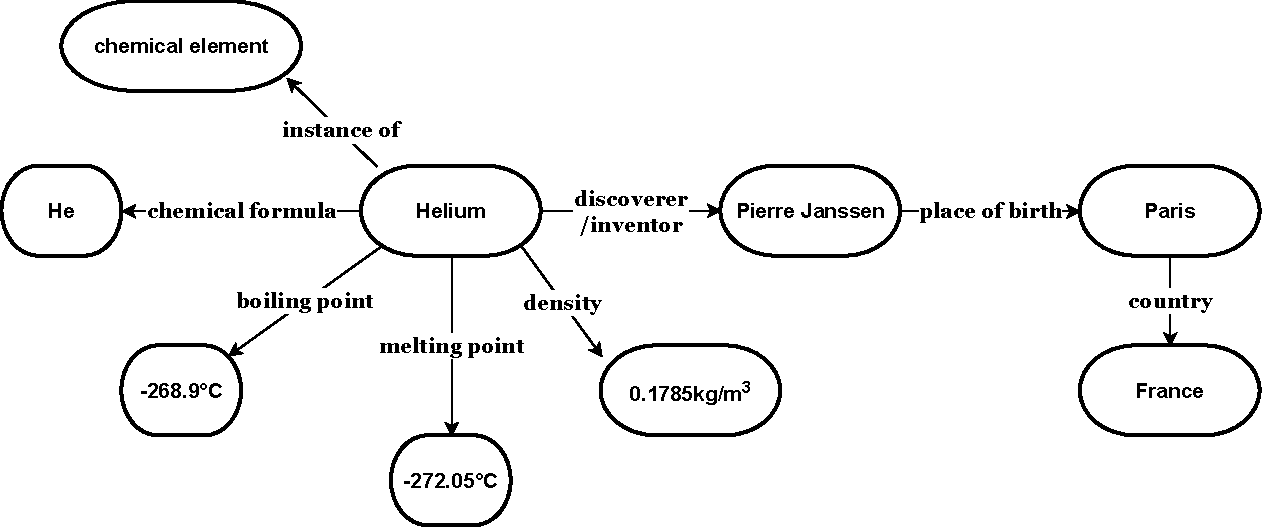
\includegraphics[width=0.80\linewidth]{images/del_graph.drawio.pdf}
  \caption{Directed edge-labelled graph describing Helium}
  \label{fig:figure 1}
\end{figure}

RDF Schema (RDFS) is the Vocabulary Description Language for RDF. Basically, it defines the vocabulary for RDF data. This means that it describes:

\begin{itemize}
	\item the basic concepts and abstract syntax of RDF such as resources and classes\footnote{https://www.w3.org/TR/rdf-concepts/ .}
	\item the formal semantics of RDF\footnote{https://www.w3.org/TR/2014/REC-rdf11-mt-20140225/ .}
	\item the different concrete syntaxes such as Triples, which is shown in section XYZ
\end{itemize}

According to RDFS, resources are divided into groups known as classes. Each member of a class is called an instance of that class, and is itself also a resource. The relationship between subject and object resources is described via RDF properties Essentially, the predicate of an RDF statement is an instance of RDF property. For instance, to identify that a resources is an instance of a class we use the predicate rdf:type which is in turn an instance of RDF property. W3cC provides a thorough documentation on RDF Schema.\footnote{w3.org/TR/2014/REC-rdf-schema-20140225/ .} In Figure 1 we see that Helium is an instance of the class chemical element. The property instance of describes the relation between the subject Helium and object chemical element.
\anas{Is the concept of property and predicate clear?}

In order to exchange graphs across the web we need to identify the resources uniquely. For this we use IRIs which are basically identifiers in RDF. The graph shown in Figure~\ref{fig:figure 1} can be represented using an RDF graph. Formally, the building blocks of RDF graphs are IRIs, literals and blank nodes. These are defined as follows.

\subsection*{IRI}
%\subsubsection{IRIs}
A Uniform Resource Identifier (\acrshort{URI}) is a sequence of a subset of ASCII characters that identifies any web resource by using a name, a location, or both. They have a scheme, authority, path, and query and fragment, where all parts other than scheme and path are optional. URIs are of the form \textbf{scheme:[//authority]path[?query][\#fragment]}. For example, \textit{http://www.wikidata.org/entity/Q560} is an IRI that identifies the chemical element Helium on Wikidata. A Uniform Resource Locator (\acrshort{URL}) is a subset of URI that is used to specify the location of a digital document.

An Internationalized Resource Identifier (\acrshort{IRI}) is a generalized form of URI that helps to distinguish resources with Unicode. Basically, the character set in URI is extended to the Universal Coded Character Set. This enables it to contain any Latin and non-Latin characters except the reserved characters.

In RDF an IRI is used as a name (can be thought of as an ID) for graph nodes. It defines the resources that appears as nodes or edge labels in a RDF graph. There are already several pre-existing IRIs available for common use. New domain specific IRIs can be created based on the application. However, we must ensure there no conflicts with other IRIs available on the web.

\subsection*{RDF Literals}
%\subsubsection{RDF Literals}

An RDF literal consists of three essential elements: a lexical value, a datatype IRI and an optional language tag. The lexical value is a string\footnote{RDF is based on Unicode strings.} that corresponds to a particular literal value in the value space, where value space is the set of all possible values that a datatype can have. There are many datatypes\footnote{A full list is available on the W3C's section on RDF datatypes: www.w3.org/TR/2014/REC-rdf11-concepts-20140225/\#section-Datatypes.} in RDF some of which are string, Boolean, decimal and integer.

The datatype IRI refers to a datatype that defines which strings are valid (belong in the lexical space), the value space and the lexical-to-value mapping \cite{ Bonduel2019}. This mapping is essentially a function that maps each string from the lexical space to an element in the value space. The \acrshort{W3C} standard XML Schema defines the datatypes and their IRIs. For example, decimals are identified by the IRI http://www.w3.org/2001/XMLSchema\#decimal. W3C has a good documentation on the different XML Schema built-in datatypes \cite{ R.Cyganiak2014}.

The optional language tag helps to provide human-readable labels to RDF literals. A literal is a language-tagged string is of the form "string"@language.\footnote{Here language is a well-formed language tag (after \acrshort{BCP47}).} The datatype IRI\footnote{It is never used in syntax.} of such literals is http://www.w3.org/1999/02/22-rdf-syntax-ns\#langString.

RDF literals are used to represent resources that have values belonging to datatypes. Each literal can have only one datatype. For example, the boiling point of Helium would be a RDF literal represented as \texttt{-268.9^^xsd:decimal} and its chemical formula as \texttt{"He"@en}, which is a language-tagged string. Literals are drawn as rectangular nodes in RDF graphs. 

\subsection*{Blank Nodes}
%\subsubsection{Blank Nodes}
A blank node in RDF, also known as a bnode, does not identify a specific resource as IRIs or literals do. It is used as a placeholder for some node, i.e., it is used to say that something with the given relationship exits at the position without specifying what the node is.


\subsection{RDF Graph}
\begin{definition}[RDF Graph]	
An RDF graph is a directed edge-labelled graph composed of a set of triples. A triple, also known as statement, represents the relationship between a subject and an object, linked by a predicate as shown in Figure~\ref{fig:figure 2}. Formally, each triple consist of the following elements:  

\begin{itemize}
	\item a subject node that is an IRI or a blank node
	\item a predicate edge that is an IRI
	\item an object node that is an IRI, a blank node, or a literal
\end{itemize}	
\end{definition}

\begin{figure}[h]
  \centering
  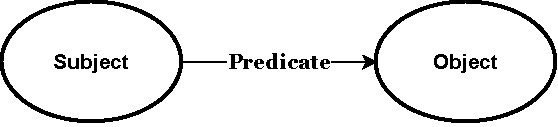
\includegraphics[width=0.75 \linewidth]{images/rdf_relation.drawio.pdf}
  \caption{An RDF graph with Subject and Object nodes connected via a predicate edge}
  \label{fig:figure 2}
\end{figure}



Figure~\ref{fig:figure 3} shows an RDF graph based on our example represented in Figure~\ref{fig:figure 1}. Our main interest is in querying the knowledge graph Wikidata, and so all the data correspond to the resources in its knowledge base. In Wikidata the subject and object represent items, and the predicate represents properties. All items and properties are identified as Unique IDs. For example, the item \textit{Helium} has the ID of \texttt{Q560}, and the property \textit{chemical formula} has the ID \texttt{P274}. These are not understood by humans and have a label property that makes them understood. Moreover, items belong to the namespace \texttt{http://www.wikidata.org/entity/} (prefixed by \texttt{wd}) and properties to \texttt{http://www.wikidata.org/prop/direct/} (prefixed by \texttt{wdt}). As a result, \textit{Helium} would have the IRI \texttt{http://www.wikidata.org/entity/Q560} (\texttt{wd:Q560}) and \textit{chemical formula} the IRI \texttt{http://www.wikidata.org/prop/direct/P274} (\texttt{wdt:P274}). Section XYZ gives an elaborate understanding of entities and the namespaces they belong to in Wikidata.

From Figure~\ref{fig:figure 3} we understand that \textit{Helium} \texttt{(\gls{Q560})} is an \textit{instance of} \texttt{(P31)} of \textit{chemical element} \texttt{(Q11344)}. It has a human understandable english \textit{label} called \textit{helium} and the \textit{chemical formula} \texttt{(P274)} of \textit{He}. Its \textit{boiling point} \texttt{(P2102)}, \textit{melting point} \texttt{(P2102)} and \textit{density} \texttt{(P2054)} are \textit{-268.9~°C}, \textit{0.1785~°C} and \textit{-272-05~kg/m3} respectively. Helium has a \textit{discoverer/inventor} \texttt{(P61)} by the name of \textit{Pierre Janssen} \texttt{(Q298581)}. His \textit{place of birth} \texttt{(P19)} was \textit{Paris} \texttt{(Q90)} that belongs to the \textit{country} \texttt{(P17)} of \textit{France} \texttt{(Q142)}.

\begin{figure}[h]
  \centering
  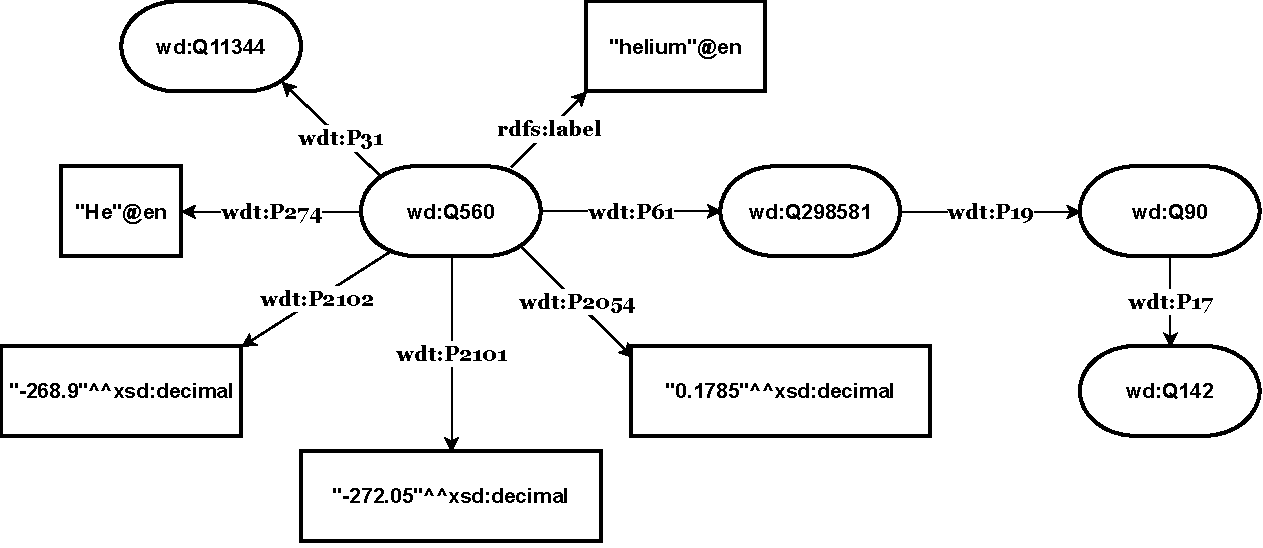
\includegraphics[width=0.75 \linewidth]{images/rdf_graph.drawio.pdf}
  \caption{RDF graph describing Helium}
  \label{fig:figure 3}
\end{figure}

%\begin{table}[b!]
%	\begin{center}
%		\caption{Abbreviation/IDs and their meanings.}
%		\label{tab: table 1}
%		\begin{tabular}{c|c}
%%			\textbf{Benchmarking tool} & \textbf{Resource monitoring tool} & \textbf{License} & \textbf{Updated} \\ \hline
%			wd & http://www.wikidata.org/entity/ \\ \hline
%			wdt & http://www.wikidata.org/prop/direct/ \\ \hline
%			rdfs & http://www.w3.org/2000/01/rdf-schema\# \\ \hline
%			Q560 & Helium \\ \hline
%			Q298581	& discoverer/inventor \\ \hline
%			Q90 & Paris \\ \hline
%			P31	& instance of \\ \hline
%			P274 & chemical formula \\ \hline
%			P2102 & boiling point \\ \hline
%			P2101 & melting point \\ \hline
%			P2054 & density \\ \hline
%			P61	& discoverer/inventor \\ \hline
%			P19	 & place of birth \\ \hline
%			P625 & coordinate location
%		\end{tabular}
%	\end{center}
%\end{table}


\subsection{Serialisations}
For exchanging graphs across the web, we need a syntactical representation of RDF. There are different formats available, the most common ones are N-Triples, Turtle, JSON-LD, RDF/XML and RDFa. In this report we focus on N-Triples and Turtle.

\subsubsection{N-Triples}
N-Triples represents RDF graphs in a simple line-based format.\footnote{Full specification available at: https://www.w3.org/TR/n-triples/ .} Every triple is encoded in a single line. The IRIs are written within pointy brackets and literals are written as lexical value\textasciicircum \textasciicircum datatype-IRI. Blank nodes are represented as \_:stringID, where stringID can be any string used to identify the blank node in the document. After every element of a triple there is a whitespace, and all the lines end with a dot. We can use comments using hash symbol after the end of every triple in a line or in a single dedicated line, and they are treated as white spaces. The files are saved with a \textit{.nt} extension.

Listing~\ref{listing:listing1} shows the representation of the RDF graph in Figure~\ref{fig:figure 3} in N-triples format. We have given line breaks for better readability.

\begin{minipage}{\linewidth}
\begin{lstlisting}[columns=fullflexible, label=listing:listing1, caption={RDF graph represented in N-triples syntax}, language=SPARQL]

<http://www.wikidata.org/entity/Q560> <http://www.wikidata.org/prop/direct/P31> 
%\phantom{<http://www.wikidata.org/entity/Q560> <http://www.}%<http://www.wikidata.org/entity/Q11344> .
		                                                
<http://www.wikidata.org/entity/Q560> <http://www.w3.org/2000/01/rdf-schema#label> 
%\phantom{<http://www.wikidata.org/entity/Q560> <http://www.}%"helium"@en .

<http://www.wikidata.org/entity/Q560> <http://www.wikidata.org/prop/direct/P274> 
%\phantom{<http://www.wikidata.org/entity/Q560> <http://www.}%"He"@en .

<http://www.wikidata.org/entity/Q560>  <http://www.wikidata.org/prop/direct/P2102> 
%\phantom{<http://www.wikidata.org/entity/Q560> <http://www.}%"-268.9"^^<http://www.w3.org/2001/XMLSchema#decimal> .

<http://www.wikidata.org/entity/Q560> <http://www.wikidata.org/prop/direct/P2101> 
%\phantom{<http://www.wikidata.org/entity/Q560> <http://www.}%"0.1785"^^<http://www.w3.org/2001/XMLSchema#decimal> .

<http://www.wikidata.org/entity/Q560> <http://www.wikidata.org/prop/direct/P2054> 
%\phantom{<http://www.wikidata.org/entity/Q560> <http://www.}%"-272.05"^^<http://www.w3.org/2001/XMLSchema#decimal> .

<http://www.wikidata.org/entity/Q560> <http://www.wikidata.org/prop/direct/P61> 
%\phantom{<http://www.wikidata.org/entity/Q560> <http://www.}%<http://www.wikidata.org/entity/Q298581> .

<http://www.wikidata.org/entity/Q298581> <http://www.wikidata.org/prop/direct/P19> 
%\phantom{<http://www.wikidata.org/entity/Q560> <http://www.}%<http://www.wikidata.org/entity/Q90> .

<http://www.wikidata.org/entity/Q90> <http://www.wikidata.org/prop/direct/P17> 
%\phantom{<http://www.wikidata.org/entity/Q560> <http://www.}%<http://www.wikidata.org/entity/Q142> . 

\end{lstlisting}
\end{minipage}

\subsubsection{Turtle}
Turtle is an easy to read representation of RDF graphs. It extends the N-Triples format by providing several simplifications.\footnote{Full specification available at: https://www.w3.org/TR/turtle/ .} We can use prefix declarations and base namespaces at the beginning of the file to shorten IRIs. Turtle allows us to avoid repetition. We can use a semicolon at the end of a line instead of a dot if we know the next line has the same subject. Consequently, the next line will only have a predicate and object omitting the subject. Also, we can use a comma at the end of a line if we know the next line will start with the same subject and predicate. Analogously, the next line will only have a an object omitting the subject and the predicate. Blank nodes are represented using only square brackets. Additionally, we can provide predicate-object pairs within the square brackets to give further triples keeping the blank node as the subject. Turtle also provides a shorthand syntax for writing numbers. Numbers of the datatype integer, decimal and double can be written without quotes and datatype-IRIs. Boolean values can be written directly as either "\textit{true}" or "\textit{false}". The files are saved with a \textit{.ttl} extension.

Listing~\ref{listing:listing2} shows the representation of the RDF graph in Figure~\ref{fig:figure 3} in Turtle format. 

\begin{minipage}{\linewidth}
\begin{lstlisting}[label=listing:listing2, caption={RDF graph represented in Turtle syntax}, language=SPARQL]

PREFIX wd: <http://www.wikidata.org/entity/>
PREFIX wdt: <http://www.wikidata.org/prop/direct/>
PREFIX rdfs: <http://www.w3.org/2000/01/rdf-schema#>
PREFIX xsd: <http://www.w3.org/2001/XMLSchema#>
PREFIX geo: <http://www.opengis.net/ont/geosparql#>

wd:Q560 wdt:P31 wd:Q11344 ;
%\phantom{wd:Q560 }% rdfs:label "helium"@en ;
%\phantom{wd:Q560 }% wdt:P274 "He"@en ;
%\phantom{wd:Q560 }% wdt:P2102 -268.9 ;
%\phantom{wd:Q560 }% wdt:P2101 0.1785 ;
%\phantom{wd:Q560 }% wdt:P2054 -272.05 ;
%\phantom{wd:Q560 }% wdt:P61 wd:Q298581 .
wd:Q298581 wdt:P19 wd:Q90 .
wd:Q90 wdt:P17 wd:Q142 .

\end{lstlisting}
\end{minipage}


\section{Wikidata}
%\subsection{Wikidata}
Wikidata is a free and publicly available knowledge base that can be read and edited by both humans and machines. It is one of the many projects by Wikimedia Foundations such as Wikipedia, Wikibooks, Wikimedia Commons and Wikitionary.  Wikidata was created in 2012 at Wikimedia Deutschland by a community of volunteers. These volunteers edit and control all content. As of December 2022, Wikidata has more 23000 active editors.\footnote{https://wikidata.wikiscan.org/ .} Wikidata provides a website where data can be viewed and also edited \cite{Foundationa}.

One of the original purposed behind the creation of Wikidata was to help its sister projects. Initially, Wikipedia and its sister projects used to maintain their own lists of interlanguage links. This refers to links between Wikipedia articles about the same topic but in different languages. After 2012, these interlanguage links were provisioned via Wikidata. Wikidata is also used to display data shown inside the pages in Wikipedia. The usage of this mainly depends on the language of the Wiki. For instance, in the case of some languages, parts of the Wikipedia pages are created automatically from the data in Wikidata. Others, especially those of smaller languages that are not widely used, use Wikidata to create placeholder pages when an article may not be in their respective language. In 2018, around 59\% of Wikidata information was used in English Wikipedia articles, although mostly for external identifiers and coordinate locations \cite{Wikipedia2017}. 

Wikidata stores information in the form of structured data in a database \cite{Tharani2021}. This is not the case for its sister projects as they contain unstructured data stored. The information on their web pages is not directly given a structure in the form of tables or lists. Wikidata acts as a central storage for these projects and focuses on providing a structure for their data \cite{Wikidata2014}. Addtionally, Wikidata also supports linked data. This means that the data stored can be linked to datasets and databases like Google Books and OmegaWiki. Wikidata can also be used for quality checks against Wikipedia articles. This is useful when information about a specific topic needs to be known and the solution is easily found by querying the knowledge graph, in this case Wikidata.

Moreover, there is also a wide range of commercial and research oriented applications for Wikidata. This is due to the fact that it has a large amount of real world data. For instance, Wikidata has external usages in many large organizations such as Eurowings, Google, Apple and Amazon. This includes tasks such as data integration, authority control, identity providing and data-driven journalism. In the field of research, Wikidata is used for collecting test data for knowledge graph related algorithms and training data for machine learning projects.

Wikidata is built on the RDF framework. However, it does not define its resources in terms of RDF. Instead, it has its own model known as Wikibase data model.\footnote{https://www.mediawiki.org/wiki/Wikibase/DataModel.} This distinction creates an abstract layer between its model and RDF. Consequently, there are similarities with RDF’s W3C standards but there are also some important differences. For instance, the Wikidata property \textit{instance of} (\texttt{P31}) is semantically equivalent to the property \textit{rdf:type} in RDF. The value of \texttt{P31} is a class that is itself an item. Wikidata offers an explanation for some of the standards properties in Wikidata that correspond to the ones in RDF \cite{Foundation}. Statements (triples) in Wikidata can have annotations (qualifiers) and references.

The basic elements in Wikidata are entities, also known as resources. These are mainly items and properties. The next section describes entities in Wikidata. 

\subsection{Entities}
Wikidata maintains its data structure by pages. Each entity has a dedicated page for itself. Basically, every element on which Wikidata has structured data is known as an entity\cite{Erxleben2014}. Entities are identified by an unique ID and not by names or labels. Currently, Wikidata has mainly three types of entities – item, property and lexeme. Other extensions can define new entity types such as MediaInfo and subentities like Form and Sense. We will discuss about items and properties. The rest are out of the scope of this report.

Items are real-world objects, concepts or events. According to RDF terminology, items are instances and classes. Instead of a human understandable name, they are identified by a QID - an ID prefixed with the letter "Q" and followed a number. Items in Wikidata belong to the main namespace - \textit{http://www.wikidata.org/wiki/QID}. Every item constitutes of the following main parts - labels, descriptions, aliases, sitelinks and statements\cite{Erxleben2014}.

Labels, descriptions and aliases are multilingual which help to find the respective item. Since items are identified by an ID, these are used to identify the items clearly. Sitelinks provide links about an individual item in Wikidata to external pages on other Wikimedia sites such as Wikipedia and its other sister projects. The most important part are statements. 

A statement in Wikidata consists of a claim, references and a rank. Claims are property-value pairs, which along with the item form a RDF triple, where the item is the subject. Claims can also contain optional qualifiers that provide some additional information for the claim. This information is a property-value pair that refers to the main part of the statement instead of the item itself\cite{Erxleben2014}. References point to resources that support the claim. An item can have several statements for the same property, and all of them might not necessarily be important or relevant. Ranks are used as a quality factor to distinguish between several statements. A Wikidata statement can have one of three types of ranks - "normal", "preferred" and "deprecated". By default, a statement has the normal rank unless changed to preferred or deprecated. A statement with preferred rank means it should be given priority over the normal ranked statements. A deprecated rank indicates that the statement is incorrect or under discussion, and it may have a reference. Deprecated statements are kept either for the sake for completion or to prevent users from constantly adding or removing them. Wikidata has around 100 million items\footnote{https://grafana.wikimedia.org/d/000000167/wikidata-datamodel.} and around 1.43 billion item statements as of December 2022.\footnote{https://grafana.wikimedia.org/d/000000175/wikidata-datamodel-statements.}

Figure~\ref{fig:figure 4} shows an excerpt of the Wikidata page on the item Helium.\footnote{https://www.wikidata.org/wiki/Q560.} We can see Helium has the QID of Q560, and has labels, descriptions and aliases in different languages. It has a sitelink for the item in Wikipedia offered in 186 languages. Helium has a statement that indicates that Helium has the instance of property with chemical element as the values. The property-value pairs follows, hydrogen and followed by, lithium are qualifiers. This statement hence gives us the information that Helium is an instance of chemical element, and it comes after the element hydrogen and if followed by the element lithium. This statement has no references and has the normal rank (indicated by the middle portion greyed).

\begin{figure}[h]
  \centering
  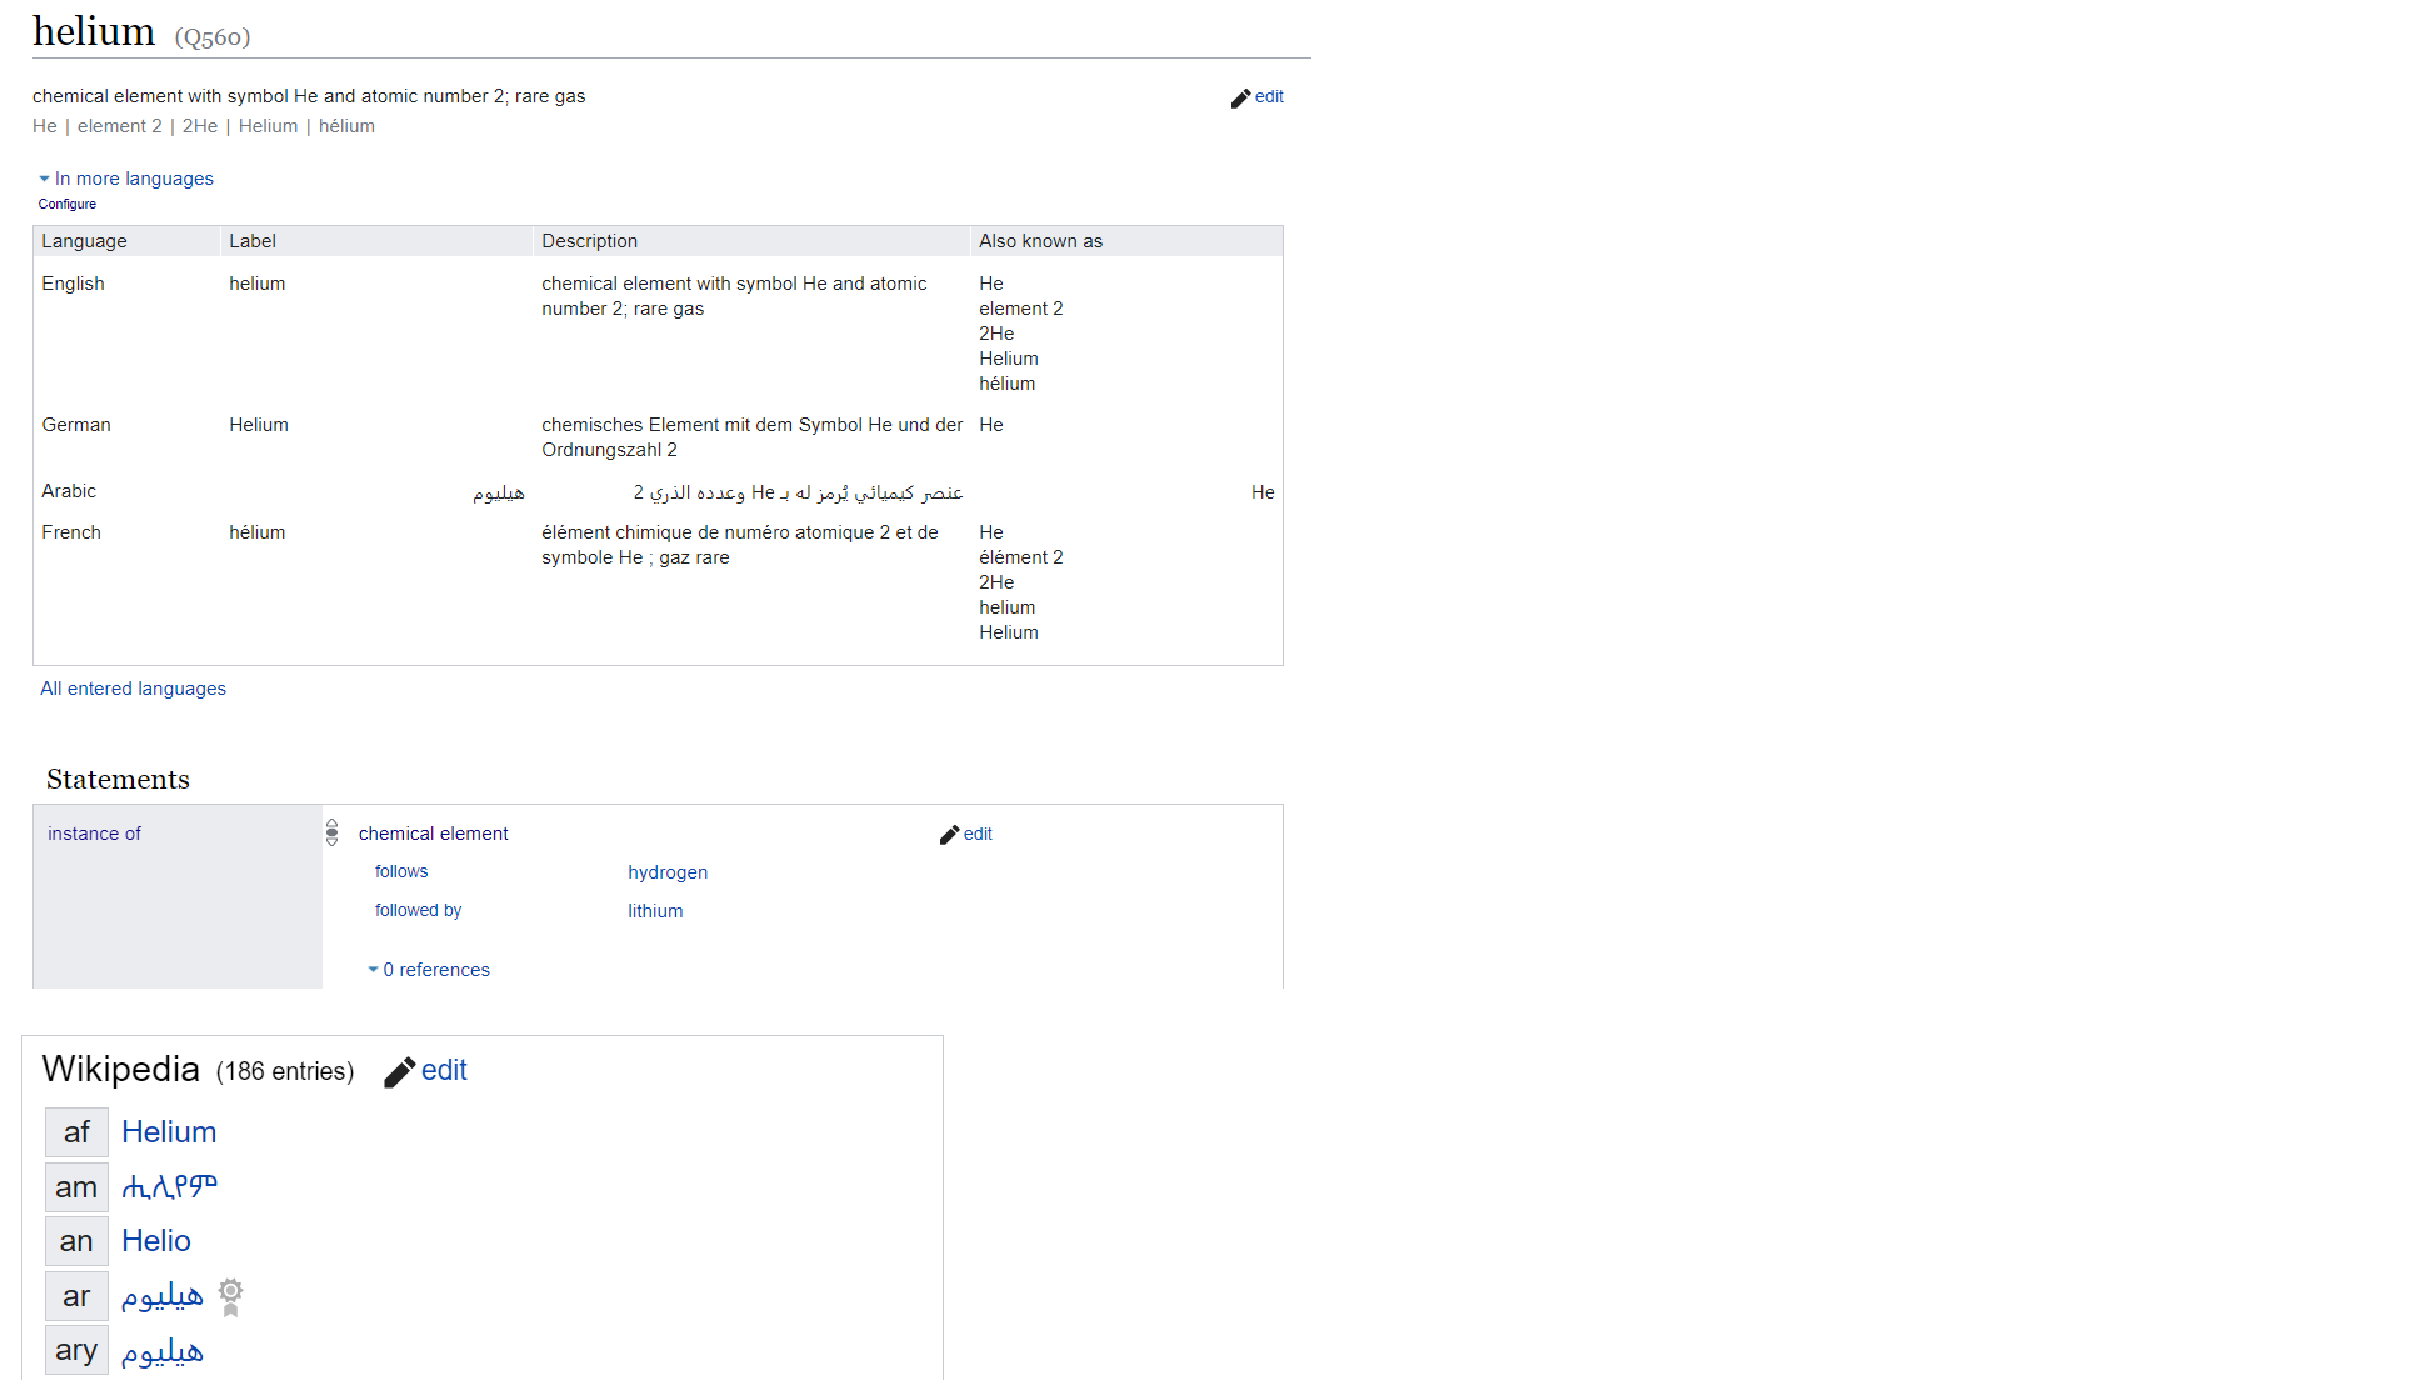
\includegraphics[width=0.75 \linewidth]{images/helium.pdf}
  \caption{An excerpt of the page on \textit{Helium} in Wikidata}
  \label{fig:figure 4}
\end{figure}

Properties in Wikidata resemble RDF properties and are essentially attributes for describing entities. They are identified by a PID - an ID prefixed with the letter "P" and followed a number. They belong to the property namespace in wikidata - http://www.wikidata.org/wiki/Property:PID. Like items, they also have labels, descriptions, aliases and statements but no sitelinks. However, they has an additional part called datatype that determines which values they accept, such as string, quantity and time.\footnote{Wikidata provides a list of all the datatypes: https://www.wikidata.org/wiki/Special:ListDatatypes.}

Figure~\ref{fig:figure 5} shows an excerpt of the property instance of page on Wikidata.\footnote{https://www.wikidata.org/wiki/P31.} The property has a PID of P31 along and with multilingual labels, descriptions and aliases. From the statement we understand that it this property also has an instance of property with Wikidata property being the value. The statement has no qualifiers or references, and has the normal rank. The instance of property accepts the datatype item as a value.

\begin{figure}[h]
  \centering
  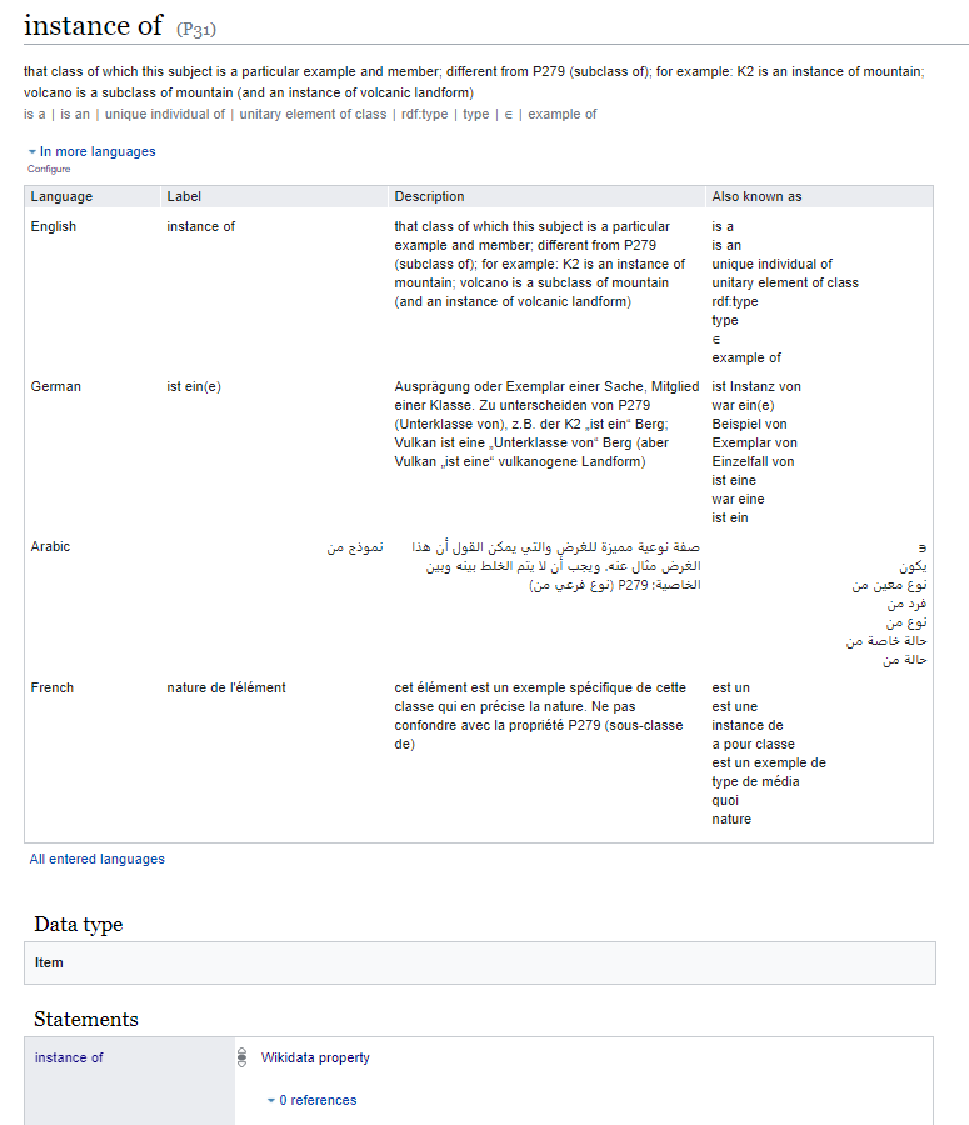
\includegraphics[width=0.75 \linewidth]{images/instance_of.pdf}
  \caption{An excerpt of the page on \textit{instance of} in Wikidata}
  \label{fig:figure 5}
\end{figure}

\subsection{Querying Wikidata}

The easiest and most popular way to query Wikidata is through the Wikidata Query Service (WDQS). This is Wikidata's SPARQL endpoint. We can use this service two ways. Firstly, we can write queries in SPARQL directly on the web user interface of the service\footnote{https://query.wikidata.org/ .} and obtain the results in different formats like table, tree, graph, etc. Secondly, the service can also be used progmatically by submitting GET or POST requests.\footnote{https://query.wikidata.org/sparql.}

Another popular way to query Wikidata is by using the Wikidata API.\footnote{https://www.wikidata.org/wiki/Special:ApiSandbox.} However, this API should mainly be used when we want to edit the contents of Wikidata or get data about entities like revision history.

Wikidata dumps is useful when we know our result set will be significantly large or if we want to set up our own local query service. These dumps are full exports of all the available entities in Wikidata.\footnote{https://dumps.wikimedia.org/ .} To get started you should download the latest complete dump.\footnote{https://dumps.wikimedia.org/wikidatawiki/latest/ .} Wikidata also mentions some other ways to accessing Wikidata's data like Search and Linked Data Fragments endpoint, the complete list and usage of which can be found on Wikidata's Data Access webpage \cite{ Wikidata2022}.


\section{SPARQL}
%\subsection{SPARQL}
SPARQL Protocol and RDF Query Language (SPARQL)\footnote{https://www.w3.org/TR/sparql11-overview/ .} is a W3C recommended query language for RDF. This means it allows to query any data source that can be mapped to RDF. It is also a HTTP-based protocol for linked open data on the web. This enables the transmission of SPARQL queries and results between a client and a SPARQL engine. The first working draft for SPARQL was released in 2004 and it became a W3C Recommendation in 2008 \cite{Perez2009}. 

Queries in SPARQL are based on matching graph patterns and can be used to retrieve, add or delete data in the RDF based dataset. In section XYZ we saw that RDF data is based on triples - subject, object and predicate. Consequently, a query in SPARQL consists of a set of triple patterns. Each of the elements of the triple can be a variable (a string beginning with ? or \$) that needs to be queried. The solution to the variables is obtained by matching the query patterns to the triples in the dataset.

There are four forms of queries - SELECT, ASK, CONSTRUCT and DESCRIBE. 
\begin{itemize}
\item SELECT queries select some or all the pattern matches and provides the results in a tabular format
\item ASK queries check whether there is at least one match and the result is true or false
\item CONSTRUCT queries create an RDF graph based on the query results
\item DESCRIBE queries return a RDF graph providing additional information on each results
\end{itemize}

In our work, we only consider SELECT queries. These consist of the following major blocks:
\begin{itemize}
\item Prologue: PREFIX and BASE keywords that function similarly to those in RDF turtle format
\item Select clause: SELECT keyword followed by either a list of variables and variable assignments, or by *
\item Where clause: WHERE keyword followed by a query graph pattern to be matched
\item Solution set modifiers: Change the set of solutions using modifiers such as LIMIT and OFFSET
\end{itemize}

The select and where clauses are mandatory, the rest being optional. Other optional features are filters, groups, query operators such as UNION, OPTIONAL and BIND, and aggregates. A full specification for the query language can be found on the official W3C documentation\cite{Seaborn}.

Listing~\ref{listing:listing3} shows an example of querying Wikidata using SPARQL. We want to get a a list of all chemical elements, along with their English labels, that have a chemical formula, boiling point, melting point, density, an inventor/discoverer, birth place of that inventor/discoverer and the country that the place belongs to. Since there might be several results, we are limiting them to five using the LIMIT keyword. The namespace http://www.wikidata.org/entity/ is used for items when querying. We are interested in the truthy values of the properties and so the namespace http://www.wikidata.org/prop/direct/ is used for properties. Truthy values are essentially the values for which the statement has the best non-deprecated rank. This means that if a statement has preferred rank then that statement is considered to be truthy. Otherwise, the normal ranked statement is taken to be truthy. The PREFIX is optional since Wikidata recognizes the short forms wd and wdt automatically. Turtle syntax that we saw in section XYZ can be applied in SPARQL. The query can be run in Wikidata's query service.\footnote{https://query.wikidata.org/ .}  

\begin{minipage}{\linewidth}
\begin{lstlisting}[label=listing:listing3, caption={Querying Wikidata with SPARQL}, language=SPARQL]

PREFIX wd: <http://www.wikidata.org/entity/>
PREFIX wdt: <http://www.wikidata.org/prop/direct/>
SELECT *
WHERE {
  ?element wdt:P31 wd:Q11344 ;
  %\phantom{?element }% wdt:P274 ?element_formula ; 
  %\phantom{?element }% wdt:P2102 ?boiling_point ;
  %\phantom{?element }% wdt:P2101 ?melting_point ;
  %\phantom{?element }% wdt:P2054 ?density ;
  %\phantom{?element }% wdt:P61 ?discoverer .
  ?discoverer wdt:P19 ?place_birth .
  ?place_birth wdt:P17 ?country .
  FILTER(LANG(?element_label)="en")
}LIMIT 5

\end{lstlisting}
\end{minipage}

Table 1 shows the results obtained in a tabular form. Among the results, there is the element Helium (Q560) that we have used as an example in Fig 1 and Fig 3. 

\begin{table}[h]
	\begin{center}
		\caption{Results of the SPARQL query in Listing 2}
		\label{tab: table 1}
		\begin{tabular}{ccccccccc}
		
%		\textbf{element} & \textbf{element_formula} & \textbf{element_label} & \textbf{boiling_point} & \textbf{melting_point} & \textbf{density} & \textbf{discoverer} & \textbf{place_birth} & \textbf{country} \\ \hline
			\toprule
			
			\textbf{element} & \textbf{element\textunderscore formula} & \textbf{element\textunderscore label} & \textbf{boiling\textunderscore point} & \textbf{melting\textunderscore point} & \textbf{density} & \textbf{discoverer} & \textbf{place\textunderscore birth} & \textbf{country} \\ 
		
			\midrule
			
			wd:Q560 & He & helium	& -268.9 & -272.05 & 0.1785 & wd:Q298581 & wd:Q90 & wd:Q142 \\
			
			wd:Q560 & He & helium & -268.9 & -272.05 & 0.1785 & wd:Q950726 & wd:Q4093 & wd:Q145 \\ 
			
			wd:Q560 & He & helium & -268.9 & -272.05 & 0.1785	 & wd:Q127959 & wd:Q623765 & wd:Q145 \\ 
			
			wd:Q670 & Si & silicon & 4271 & 2570	& 2.329	& wd:Q151911 & wd:Q1451001 & wd:Q34 \\ 
			
			wd:Q568	& Li & lithium	& 1317	& 180.5	& 0.535	& wd:Q313568 & wd:Q10495519 & wd:Q34 \\
			
			\bottomrule

		\end{tabular}
	\end{center}
\end{table}

\section{GraphQL}

GraphQL (Graph Query Language) is an open source query language for APIs (Application Programming Interfaces) and a runtime for executing those queries against existing data. It describes data structured in a graph format – a collection of objects (nodes) connected to each other by some kind of relationships (edges). Runtime is usually implemented by a server.

GraphQL is usually served over HTTP through a GraphQL server. A GraphQl server consists of two main parts – schema and resolver. The API developers create a schema that is strictly typed and describes all the possible data a client can query using the service. The schema specifies object types and fields along with operations on those types. The object type represents the kind of object that can be requested by a client. 

There are three operations types – query, mutation and subscription.  We look at the query operation in this chapter; the other two are outside the scope of this report. Queries are used to fetch or read data. When compared to REST (Representational State Transfer),  queries operations in GraphQL are similar to GET requests. A resolver in GraphQL server is a function that is associated with every field and contains instructions on how to process that particular field. In other words, the resolver is responsible for retrieving a value from the data source. 

GraphQL is data agnostic, i.e., it is not concerned where the data source is located. The data could be stored in any source such as a database or a micro-service as shown in Figure XYZ. With a single API call, GraphQL can aggregate data from multiple sources and resolve the data to the client. This is one of the advantages GraphQL has over REST API where the latter would require several HTTP calls to access data from multiple sources. Apart from being data agnostic, GraphQL is also language agnostic. This means that GraphQL services, such as the schema and resolvers, can be written in any programming language such as JavaScript or Python. 

For the sake of human readability, GraphQL specification has its own Schema Definition Language (SDL). It is simple to write and understand schemas in SDL, and is similar to the language that we use to write queries. Listing XYZ shows a schema written in SDL. This schema can be in the GraphQL server against which clients can send queries for instances of chemical elements that have a name, chemical formula and boiling point. The exclamation mark means that the corresponding field is non-nullable and it is expected that GraphQL will give a value when the field is queried. A complete guide on schemas and types can be found on the official documentation from GraphQL.\footnote{https://graphql.org/learn/schema/ .} 

\begin{minipage}{\linewidth}
\begin{lstlisting}{gql.py:GraphqlLexer -x}[label=listing:listing4, caption={Schema used to query a chemical element}]
type Query{
	chemicalElement: ChemicalElement
}

type ChemicalElement{
	name: String!
	chemicalFormula: String!
	boilingPoint: Float!
}

\end{lstlisting}
\end{minipage}

Listing XYZ shows a query that can be used against this schema and the results that could be obtained. The results obtained are in JSON format. The official GraphQL website provides a comprehensive documentation on querying a GraphQL server. \footnote{ https://graphql.org/learn/queries/ .} 

\begin{minipage}{\linewidth}
\begin{lstlisting}[label=listing:listing5, caption={Query to fetch chemical elements and their properties}]
query QueryChemicalElement (limit 2){
    chemicalElement{
		name
		chemicalFormula
		boilingPoint
	}
}
\end{lstlisting}
\end{minipage}

\begin{minipage}{\linewidth}
\begin{lstlisting}[label=listing:listing5, caption={Query to fetch chemical elements and their properties}]
{
	"data":{
		"chemicalElement":{
			"name": "helium",
			"chemicalFormula": "He",
			"boilingPoint": -268.9
		},
		{	
			"name": "silicon",
			"chemicalFormula": "Si",
			"boilingPoint": 4271
		}
	}
}

\end{lstlisting}
\end{minipage}

\section{GraphQL vs SPARQL}

GraphQL and SPARQL are query languages developed with different goals in mind. GraphQL was designed mainly to wrap REST APIs in a graph like shape. This would allow fetching related data in a single request with the aid of schemas. In REST API, the same would require calling multiple endpoints. SPARQL, on the other hand, was developed mainly as a query language for RDF graphs.

SPARQL is immensely popular in the field of research and academia. However, it has not seen much growth in commercial applications. GraphQL, on the other hand, is more popular among software and web developers. There are some valid reasons for this.  

Firstly, many developers are still not familiar with the Linked Data model of RDF and SPARQL. They are more used to working with technologies such as GraphQL and RESTAPIs. Secondly, GraphQL is simple to learn and work with since it has human-oriented syntax. Among other things, this benefits application development. SPARQL however, proves to be more complex. It has more syntactic verbosity owing to the descriptive nature of writing queries. The produced output from SPARQL queries contains a lot of unnecessary metadata that is not useful for web developers and need to be further parsed for using in web applications \cite{Lisena2018}. 

Moreover, retrieval of data from knowledge graphs using SPARQL is time consuming and proves to be a steep learning curve, the reason being that there is limited documentation available for proper ontology descriptions and examples of using queries for SPARQL endpoints \cite{Angele2022}. One of the other reasons for using GraphQL over SPARQL is that developers are more equipped in using nested objects that GraphQL offers \cite{Taelman2018}. They lack the experience to work with triples which is the main foundation of SPARQL. Moreover, fewer supporting tools like libraries and frameworks exist for working and developing with SPARQL than with GraphQL \cite{Taelman2018}. 

On the other hand, SPARQL also has some advantages over GraphQL. SPARQL queries represent full graphs while those of GraphQL represent trees \cite{Taelman2018}. This make SPARQL more expressive. RDF provides a system to build detailed structures from the meaning of data, and is hence more complete and capable than GraphQL schemas \cite{Dresslar2019}. Since SPARQL works with the schema organization of RDF, this makes it more powerful than GraphQL. With SPARQL we can write complex queries that can be used to retrieve or modify data \cite{Angele2022}. As a result it is capable to satisfy many complex use cases.

Also since GraphQL alone has no notion of semantics \cite{Taelman2018}, a schema needs to be defined by the GraphQL API developers for every interface they want the client to query. This makes it difficult to integrate data returned when querying multiple different sources. SPARQL however supports federated queries which makes it more powerful and rich. Lastly, when using GraphQL we cannot uniquely identify resources on the web but which is possible using URIs with SPARQL. In other words, GraphQL has no notion of global identifiers \cite{Taelman2018}.

\textcolor{red}{Talk also about differences in terms of complexity and expressivity (mathematical, theory, semantics). Read papers: Semantics and Complexity of GraphQL, Defining Schemas for Property Graphs by using the GraphQL Schema Definition Language}


\pagebreak

\chapter{Approaches for Querying RDF Graphs with GraphQL}

In this chapter, we focus on ways of querying RDF Graphs using GraphQL. A GraphQL query has a tree-like structure. To traverse the query we can follow this tree structure, i.e., we can go up to a parent node, down to a child node or left/right to a sibling node \cite{Perez2009}. This imitates the graph structure of by RDF data.

In section XYZ of the previous chapter, we highlighted the differences between GraphQL and SPARQL. SPARQL has advantages over GraphQL, like being more expressive owing to basic graph patterns. However it has come limitations. Considering these limitations along with the advantages that GraphQL has over SPARQL, GraphQL seems to be a prospective choice to querying RDF Graphs.  For instance, the verbosity and the steep learning curve of SPARQL pose a challenge to developers in working with SPARQL. Also, the limited availability of libraries and frameworks for implementing SPARQL in applications creates a significant obstacle. 

In recent years, there have been attempts at providing approaches to querying linked data represented by RDF via GraphQL. This gave rise to several commercial and open-source solutions. Most notable ones include:

\begin{itemize}
	\item Stardog
	\item TopBraid EDG
	\item Ontotext Platform
	\item \textcolor{red}{GraphQLSPARQL} \anas{also include this later if possible}
	\item GraphQL-LD
	\item HyperGraphQL

\end{itemize}

Stardog\footnote{https://www.stardog.com/} is a commercial solution that offers a graph database called "Enterprise Knowledge Graph platform"\cite{Angele2022}. The initial versions only allowed querying their stored data using SPARQL. The support for querying using GraphQL was later added with the release of version 5.1. This solution allows users to provide a GraphQL schema. However, this is optional. When provided it can be used for translating GraphQL terms to RDF. The schema also helps in introspection purposes and for validating queries with the given typing information \cite{Gleim2020}. Introspection refers to querying GraphQL schema to find out the queries it supports. Moreover, schema also helps to limit the parts in the graph available to users, i.e., the user is only allowed to query some sections of the data available in the graph. If no schema is provided, then the conversion from GraphQL terms to RDF is done using the default namespace in that graph and can be overridden using the @prefix declarative inside the GraphQL queries \cite{Taelman2019}. However, this option requires the user to have a good knowledge about the way data is structured in the graph database. Introspection, data validation and access control is not possible when there is no schema \cite{Gleim2020}. In Stardog the top level node, also known as parent node, is considered to refer to a type. Any subsequent child nodes refer to the predicate links from the parent node \cite{Taelman2019}. This is an important distinction not necessarily shared by the other approaches.

TopBraid Enterprise Data Governance (TopBraid DG) is also a commercial solution created by TopQuadrant\footnote{https://www.topquadrant.com/} to query RDF graphs using GraphQL. It uses GraphQL schemas that can be automatically generated based on SHACL\footnote{https://www.w3.org/TR/2017/REC-shacl-20170720/} \cite{Taelman2019}. With the generation of schema, introspection also becomes possible. One important feature of TopBraid EDG is the functionality of query mutation. This allows the users to modify existing data in the graph.

Ontotext Platform\footnote{https://www.ontotext.com/products/ontotext-platform/} is a commercial solution offered by Ontotext. Users are provided with a GraphQL interface that they can to query the underlying graph database called "GraphDB" \cite{Angele2022}. 

The above mentioned proprietary solutions are not open source and only allow querying their corresponding graph databases. This implies they cannot be used to query arbitrary knowledge graphs such as Wikidata, which is the focus of this report.

GraphQL-LD and HyperGraphQL are two open source solutions that can be used to query knowledge graphs that provide a SPARQL endpoint. We present in details about them in the following sections.

\section{GraphQL-LD}

GraphQL-LD originates from an ongoing research work proposed by \citeauthor{Taelman2018} to query knowledge graphs via GraphQL \cite{Taelman2018}. The main working process behind this is to extend the GraphQL queries with JSON-LD context to fetch RDF data. 

JSON (Java Script Object Notation) is a widely popular data exchange format used for storing and sending information over the internet. JSON-LD (JavaScript Object Notation for Linked Data) is a syntax used to serialize Linked Data in JSON. It is also a W3C Standard. JSON-LD provides features such as identifying JSON objects by IRIs and annotating strings with their language. The official documentation for JSON-LD provided by W3C gives a detailed explanation of its features \cite{Sporny2014}. JSON-LD context is used to map terms into IRIs. It allows the data exchanged to be unambiguous globally in the sense that it can be meaningful to anyone receiving it on the web.   

The GraphQL query selects the data (nested in fields) that we want to fetch. The JSON-LD context maps the query fields to URIs. In other words, it helps to provide a link between the items in the nodes of the queries and the actual resources that exist in the respective Linked Data source. The GraphQL queries are then converted into SPARQL queries that can be used to query any source consisting of Linked Data and a SPARQL endpoint.

Listing XYZ and Listing XYZ shows an example where a query coupled with JSON-LD context can be used to fetch RDF data from a RDF data source - http://example.org\footnote{This domain is for use in illustrative examples in documents}. The JSON-LD context helps to identify the resources - chemicalElement, name, chemicalFormula and boilingPoint – by providing an unique IRI specific to those resources in the RDF data source.

\begin{minipage}{\linewidth}
\begin{lstlisting}[label=listing:listing6, caption={GraphQL query}]
{
	chemicalElement {
		name
		chemicalFormula
		boilingPoint
	}
}
\end{lstlisting}
\end{minipage}

\begin{minipage}{\linewidth}
\begin{lstlisting}[label=listing:listing7, caption={JSON-LD context}]
"@context": {
	"chemicalElement": "http://example.org/chemicalElement",
	"name": "http://example.org/name",
	"chemicalFormula": "http://example.org/chemicalFormula",
	"boilingPoint": "http://example.org/boilingPoint"
}
\end{lstlisting}
\end{minipage}

The approach taken by GraphQL-LD consists primarily of two standalone modules:
\begin{itemize}
	\item \textbf{GraphQL to SPARQL algebra}: Parses a GraphQL query to SPARQL algebra expression
	\item \textbf{SPARQL results to tree}: Converts a SPARQL query result into a tree structure
\end{itemize}


\subsection{GraphQL to SPARQL algebra}

The "GraphQL to SPARQL algebra" module is used for parsing a GraphQL query into an expression in SPARQL algebra\footnote{https://www.w3.org/TR/sparql11-query/\#sparqlQuery.} with the help of a JSON-LD context. A SPARQL algebra expression is is formed from parsing the strings in SPARQL query followed by some transformations. It is basically used to provide semantics to the syntax in SPARQL query.

The algorithm for the conversion of GraphQL query to SPARQL algebra expression is based on translating the tree-like structure of GraphQL to links of triple patterns or statements  in SPARQL \cite{Taelman2018}. Listing XYZ shows the SPARQL algebra obtained by parsing the GraphQL query in Listing XYZ.

\begin{minipage}{\linewidth}
\begin{lstlisting}[label=listing:listing8, caption={Generated SPARQL Algebra}]
{
  type: 'project',
  input: { type: 'bgp', patterns: [ [Quad], [Quad], [Quad], [Quad] ] },
  variables: [
    Variable { termType: 'Variable', value: 'chemicalElement_name' },
    Variable {
      termType: 'Variable',
      value: 'chemicalElement_chemicalFormula'
    },
    Variable {
      termType: 'Variable',
      value: 'chemicalElement_boilingPoint'
    }
  ]
}

\end{lstlisting}
\end{minipage}

The Quads are listed in Listing XYZ:

\begin{minipage}{\linewidth}
\begin{lstlisting}[label=listing:listing9, caption={The expansion of Quads}]
[
  Quad {
    termType: 'Quad',
    value: '',
    subject: Variable { termType: 'Variable', value: 'df_3_0' },
    predicate: NamedNode {
      termType: 'NamedNode',
      value: 'http://example.org/chemicalElement'
    },
    object: Variable { termType: 'Variable', value: 'chemicalElement' },
    graph: DefaultGraph { termType: 'DefaultGraph', value: '' },
    type: 'pattern'
  },
  Quad {
    termType: 'Quad',
    value: '',
    subject: Variable { termType: 'Variable', value: 'chemicalElement' },
    predicate: NamedNode {
      termType: 'NamedNode',
      value: 'http://example.org/name'
    },
    object: Variable { termType: 'Variable', value: 'chemicalElement_name' },
    graph: DefaultGraph { termType: 'DefaultGraph', value: '' },
    type: 'pattern'
  },
  Quad {
    termType: 'Quad',
    value: '',
    subject: Variable { termType: 'Variable', value: 'chemicalElement' },
    predicate: NamedNode {
      termType: 'NamedNode',
      value: 'http://example.org/chemicalFormula'
    },
    object: Variable {
      termType: 'Variable',
      value: 'chemicalElement_chemicalFormula'
    },
    graph: DefaultGraph { termType: 'DefaultGraph', value: '' },
    type: 'pattern'
  },
  Quad {
    termType: 'Quad',
    value: '',
    subject: Variable { termType: 'Variable', value: 'chemicalElement' },
    predicate: NamedNode {
      termType: 'NamedNode',
      value: 'http://example.org/boilingPoint'
    },
    object: Variable {
      termType: 'Variable',
      value: 'chemicalElement_boilingPoint'
    },
    graph: DefaultGraph { termType: 'DefaultGraph', value: '' },
    type: 'pattern'
  }
]
\end{lstlisting}
\end{minipage}

It is also possible to view the generated SPARQL queries using a CLI tool - "graphql-to-sparql". The generated SPARQL query for our example is shown in Listing XYZ.

\begin{minipage}{\linewidth}
\begin{lstlisting}[label=listing:listing10, caption={Genertaed SPARQL query}]
SELECT ?chemicalElement_name ?chemicalElement_chemicalFormula ?chemicalElement_boilingPoint WHERE {
  ?df_3_0 <http://example.org/chemicalElement> ?chemicalElement.
  ?chemicalElement <http://example.org/name> ?chemicalElement_name;
    <http://example.org/chemicalFormula> ?chemicalElement_chemicalFormula;
    <http://example.org/boilingPoint> ?chemicalElement_boilingPoint.
}
\end{lstlisting}
\end{minipage}

GraphQL-LD offers many of the functionalities that are listed in the official documentation of GraphQL\footnote{https://graphql.org/learn/queries/ .} such as fragments, directives and aliases. However, triple patterns are not sufficient to express all of these features\cite{Taelman2018}. For example, for the fragments feature in GraphQL, GraphQL-LD uses the left-join semantics. This translates to the OPTIONAL keyword in SPARQL.

Along with the "@include" and "@skip" directives\footnote{https://graphql.org/learn/queries/\#directives.} included in the core GraphQL specification, GraphQL-LD offers three custom directives as well to further enrich the queries - "@optional", "@single" and "plural". In GraphQL-LD all fields in the query are required to have results. In the event that any of the fields does not return a result, the entire result set will return as empty. When we are uncertain about a field returning a result we can use the "@optional" custom directive with that field. Basically, this custom directive allows the users to specify the fields that are optional. The module converts the directive to the OPTIONAL operator in SPARQL. We will discuss about the "@singular" and "plural" custom directive in the next section.

A comprehensive information on the conversion from GraphQL queries to SPARQL queries is available under the "graphql-to sparql.js" GitGub repository.\footnote{https://github.com/rubensworks/graphql-to-sparql.js}

\subsection{SPARQL results to tree}

The "SPARQL results to tree" module converts the SPARQL query results into a tree-based structure constituting of plain JSON objects. This is convenient since the user writes the queries in a tree-like fashion in GraphQL and expects the results to be in the same structure.

After a generated SPARQL query is sent to the Linked Data interface, such as a SPARQL endpoint, the results are returned as SPARQL JSON. This is what is meant by the SPARQL query results. This "SPARQL results to tree" module converts these results into a tree-based structure based by splitting the variable names based on a certain delimiter value. The default delimiter value used in GraphQL-LD is an underscore. This gives rise to paths inside the tree structure.

Listings XYZ and XYZ show an example SPARQL result and its conversion to the tree-based structure respectively.

\begin{minipage}{\linewidth}
\begin{lstlisting}[label=listing:listing11, caption={SPARQL Algebra result}]
{
  "results": {
    "bindings": [
      { "chemicalElement_name": { "type": "literal", "value": "Helium" }, "chemicalElement_chemicalFormula": { "type": "literal", "value": "He" }, "chemicalElement_boilingPoint": { "type": "literal", "value": "-268.9" } },
      { "chemicalElement_name": { "type": "literal", "value": "Silicon" }, "chemicalElement_chemicalFormula": { "type": "literal", "value": "Si" }, "chemicalElement_boilingPoint": { "type": "literal", "value": "4271" } }
    ]
  }
}
\end{lstlisting}
\end{minipage}

\begin{minipage}{\linewidth}
\begin{lstlisting}[label=listing:listing12, caption={Tree-based JSON result}]

{
"chemicalElement":[
	{ "name": "Helium", "chemicalFormula": "He", "boilingPoint": "-268.9" },
	{ "name": "Silicon", "chemicalFormula": "Si" , "boilingPoint": "-4271"  }
	]
}

\end{lstlisting}
\end{minipage}

When writing a GraphQL query, we can decide whether the values obtained from querying should be wrapped in array or not, using the custom directives "@singluar" and "@plural" respectively on the fields. GraphQL-LD assigns all fields to be plural by default. This is a convenient feature\footnote{https://github.com/rubensworks/graphql-to-sparql.js/\#converting-to-tree-based-results.} that allows the results to be compacted.

A comprehensive information on the conversion from SPARQL results to tree-strcuture is available under the "sparqljson-to-tree.js" GitGub repository.\footnote{https://github.com/rubensworks/sparqljson-to-tree.js}

The basic overview is that GraphQL-LD takes a GraphQL query and a JSON-LD context from the user and converts the query into a SPARQL query. This generated SPARQL query is sent to a Linked Data interface such as a SPARQL endpoint for execution. We can also use this to query our own own local Linked Data files instead of a remote endpoint. Finally, the obtained query results from the endpoint are then converted into a tree-based structure corresponding to the original GraphQL query. Figure XYZ shows an overview of this approach. Here we show the SPARQL endpoint as the interface being queried. The modules in GraphQL-LD are implemented in TyperScript and JavaScript, and thus can be used in Javascript applications.

GraphQL-LD is predicate-oriented. This means that it focuses on querying the relationships between the subject and object \cite{Werbrouck2019a}. This imposes a problem for implementing subject-based queries when we want to query for a specific class. An example for this would be querying for an item that is of type chemical element. To overcome this problem we would need a workaround. However, this makes the query complicated to write. In the next chapter where we implement querying Wikidata using GraphQL-LD, we discuss three workarounds that can used when we want to implement subject-based queries. 

Since GraphQL-LD is schema-less, it not possible to perform introspection\footnote{https://graphql.org/learn/introspection/ .} -  querying a GraphQL schema for information about the supported queries - since the user is not aware of the data's schema \cite{Gleim2020}. However, this is not necessary since all exposed Linked Data can be queried with GraphQL-LD \cite{Werbrouck2019a}. When writing queries, GraphQL-LD users would need to have a good understanding of the data scheme of the queried RDF data.  


\section{HyperGraphQL}

HyperGraphQL is open source GraphQL interface for querying Linked Data on the Web. It is developed and maintained by Semantics integration Ltd. The project is written in Java, with the initial release being in 2018. At the time of this writing, the latest version, 3.0.1, was released in 2021.

In addition to querying RDF data, HyperGraphQL is designed to support federated querying over multiple RDF stores via a single GraphQL query interface \cite{Taelman2019}. Federated queries refer to querying multiple data sources and combining the data. This enriches the results with interesting information as the data is obtained from various sources rather than just one. However, federated querying is challenging. Retrieving and combining data from different services requires deep understanding of the involved datasets, and different configuration parameters such as authentication need to be considered. 

A service need to be set up that acts as an intermediary server between the client side, where the GraphQL query is written, and the RDF datastore, from where Linked Data is fetched \cite{Taelman2018} . We can create multiple instances of HyperGraphQL where each instance can query one or more RDF sources, depending on the type of Linked Data services selected. In the next section we discuss these services in detail. To set up a HyperGraphQL instance two input files need to be provided - a configuration JSON file and an annotated GraphQL schema.

\subsection{Configuration File}

The configuration file contains the specifications of the RDF services from there data needs to be fetched. It includes the name of the instance, path of the GraphQL schema, HTTP settings of the instance and the specifications of the Linked Data services needed to fetch data. HyperGraphQL currently offers three types of Linked Data services: SPARQLEndpointService, LocalModeSPARQLService and HGraphQLService. 

The SPARQLEndpointService refers to the SPARQL endpoint service where data is fetched from remote RDF sources, like Wikidata and DBpedia. LocalModeSPARQLService allows to fetch data from RDF files that exists on the local system or in a remote location. \textcolor{red}{These are loaded into local memory to be used once the HyperGraphQL instance runs}. These files contain data stored as RDF triples and follow the RDF serialization format of RDF/XML, Turle or N-Triples. Lastly, the HGraphQLService allows to query data from other HyperGraphQL instances running on a server.

Listing XYZ shows a configuration file for fetching data from example.org through the SPARQLEndpointService.

\begin{minipage}{\linewidth}
\begin{lstlisting}[label=listing:listing13, caption={An example configuration file}]
{
    "name": "example-hgql",
    "schema": "schema/schema_example.graphql",
    "server": {
        "port": 8081,
        "graphql": "/graphql",
        "graphiql": "/graphiql"
    },
    "services": [
        {
            "id": "example-sparql",
            "type": "SPARQLEndpointService",
            "url": "http://example.org/sparql/",
            "graph": "",
            "user": "",
            "password": ""
        }
    ]
}
\end{lstlisting}
\end{minipage}

\subsection{Annotated Schema}

HyperGraphQL works with a GraphQL schema that needs to be defined to set up an instance. This is different from GraphQL-LD, where no schema is required. A schema gives control to the data that be queried. The user can only fetch data for the types and queries defined in the GraphQL schema \cite{Gleim2020}.

The schema contains a designated type called "\_Context". This contains the annotations that encode the mappings from every type and field in the schema to the corresponding IRI in the RDF source. The IRI should be unique and will be used to fetch data from the source. 

Each type and field in the schema is annotated with GraphQL directives that tell the instance about the service from where data for the type and filed should be fetched. These are essentially pointers or service ids that correspond to the RDF services defined in the configuration file.

Only the types annotated with a service id can be queried. Non-annotated typed will not be queryable. However, all fields need be annotated with a service id. For every annotated type, two query fields are automatically exposed - TypeName\_GET, parametrized with the "limit:Int" and "offset:Int" argument, and TypeName\_GET\_BY\_ID, parameterized with "uris:[String]" argument. Two additional fields are also introduced automatically for each type in the schema - "\_id:String" field which returns the IRI of the resource and "\_type:String" field which returns the "rdf:type" of the parent type of the resource in the schema. Moreover, every field in the schema with the value type String is provided with a "lang:String" argument by default. This allows the user to specify the language of the fetched literal.

Listing XYZ shows a GraphQL schema that can be used to query data from example.org, using the configuration file in Listing XYZ. The id:"example-sparql" in the @service directory is the same as the id in the services block of the configuration file.


\begin{minipage}{\linewidth}
\begin{lstlisting}[label=listing:listing14, caption={An example schema}]
type __Context {
    ChemicalElement:    _@href(iri: "http://example.org/chemicalElement")
    name:               _@href(iri: "http://example.org/name")
    chemicalFormula:   _@href(iri: "http://example.org/chemicalFormula")
    boilingPoint:       _@href(iri: "http://example.org/boilingPoint")
}

type ChemicalElement @service(id:"example-sparql") {
    name: String @service(id:"example-sparql")
    chemicalFormula: String @service(id:"example-sparql")
    boilingPoint: String @service(id:"example-sparql")
}
\end{lstlisting}
\end{minipage}

Like GraphQL-LD, HyperGraphQL also converts GraphQL queries into SPARQL. However, unlike GraphQL-LD where the conversion takes place on the client side, in HyperGraphQL the conversion takes place on the server side, thereby decreasing the computation overhead on the client side. Also, the generated SPARQL queries are not necessarily part of the user interaction, and are not displayed. We discuss in the next chapter when we implement HyperGraphQL to query Wikidata, the method we used to observe the generated SPARQL queries whenever an instance is set up.

Listing XYZ shows the GraphQL query we used in the section for GraphQL-LD. This query combined the schema in Listing XYZ generates the following SPARQL query in Listing XYZ.


\begin{minipage}{\linewidth}
\begin{lstlisting}[label=listing:listing15, caption={An example query}]
{
	chemicalElement {
		name
		chemicalFormula
		boilingPoint
	}
}
\end{lstlisting}
\end{minipage}


\begin{minipage}{\linewidth}
\begin{lstlisting}[label=listing:listing16, caption={The generated SPARQL query}]
SELECT * WHERE { 
	{ 
   		SELECT ?x_1 WHERE { 
    		?x_1 http://www.w3.org/1999/02/22-rdf-syntax-ns#type http://example.org/chemicalElement . 
		}  
 	}  
 	OPTIONAL { 
 		?x_1 <http://example.org/name> ?x_1_1 . 
 	}  
	OPTIONAL { 
		?x_1 <http://example.org/chemicalFormula> ?x_1_2 . 
	}  
	OPTIONAL { 
		?x_1 <http://example.org/boilingPoint> ?x_1_3 . 
	}  
}
\end{lstlisting}
\end{minipage}

We discussed in the previous section we discussed that in GraphQL-LD implementation, the result set is empty if any of the fields does not fetch a result (if the optional tag is not given to the field in the GraphQL query). With HyperGraphQL this is relaxed since the fields are translated into optional SPARQL triple patterns. We will discuss the differences between the queries generated with GraphQL-LD and HyperGraphQL in detail in chapter XYZ.

Once the instance runs on the local server, a GraphiQL\footnote{https://github.com/graphql/graphiql.} interface is created. This is the basically a graphical user interface where the user can write GraphQL queries and send them to the HyperGraphQL instance running on the local server. The instance queries the RDF data and returns a response in JSON-LD enhanced with JSON-LD context. Other RDF serialization formats are also supported for the returned response like json+rdf+xml and json+turtle. 


%\section{GraphQL-LD}
%\subsection{JSON-LD}
%Elaborate on concrete JSON-LD represetation
%\subsection{Using Graphql-LD with Wikidata}
%
%\section{HypergraphQL}
%\subsection{Schema}
%Elaborate on schema of HypergraphQL
%\subsection{Using HypergraphQL with Wikidata}
%
%\section{GraphQL vs generated SPARQL queries}
%
%\section{Differences between the generated SPARQL queries by both tools}
%
%\section{Performance Evaluation}
%1. Evaluate performance of both approaches by writing SPARQL queries and equivalent GraphQL queries \\
%2. Discuss in how far the generated Sparql queries differ from the handwritten ones. \\
%3. analyze how well the approach scales with larger (deeper) GraphQL queries.
%
%
%
%
%
%\section{Effort for the setup}
%Evaluate/discuss the effort for the setup of both tools 
%
%\section{Default context}
%
%\section{Repository}
%
%
%\section{Challenges faced and Conclusion}
%\lipsum[1]

%\appendix
\singlespacing
\bibliographystyle{splncs04}
\bibliography{main}


\printglossaries
\end{document}
